\chapter{Artifact Detection and Localization}

The artifact detection and localization pipeline is responsible for converting the sensor data from the various payloads (Mk. 0, Mk. 1, drone), into a list of artifacts to send to the base station and ultimately report to DARPA. The pipeline was developed to meet a set of requirements, which were derived from the competition rules and our team's concept of operations:

\begin{enumerate}
	\item Reported coordinate of artifact must be within 5m (Euclidean distance) of DARPA-surveyed coordinate
	\item Pipeline must run on-board, either on the Xavier (Mk. 0, Mk. 1), or on part of the NUC (drone)
	\item Artifacts must be transmitted to base station over a lossy wireless link
	\item Pipeline should be capable of detecting all 5 types of artifacts (as shown in Figure \ref{tunnel artifacts})
	\item All artifacts which the robots pass by should be detected
	\item Pipeline should be identical or nearly identical on all payloads
	\item Artifacts should be detected and reported to human supervisor in real-time
\end{enumerate}

Additionally, the following assumptions were made to constrain the scope of the pipeline and guide parameter tuning wherever necessary:

% TODO(vasua): Turn this (and above) into a table
\begin{enumerate}
	\item State estimation system on all payloads would be LOAM
	\item Artifact detection and localization pipeline could not direct robots' exploration
	\item Artifacts are reported in robots' own frames and transformed to a single world frame at base station
	\item Robots will move at approximately 2 m/s
	\item A human supervisor would be available to verify artifact reports, and thus false positives are acceptable
\end{enumerate}

An overview of the complete pipeline is given in Figure \ref{software_overview}. This pipeline runs identically on all 3 payloads with only minor configuration changes (e.g. sensor serial numbers), and sensor omissions where necessary (e.g. drone payload does not contain a thermal camera). All robots report artifacts to the GUI independently, and no information is shared between pipelines running on individual payloads.

\begin{figure}	
	\centering
	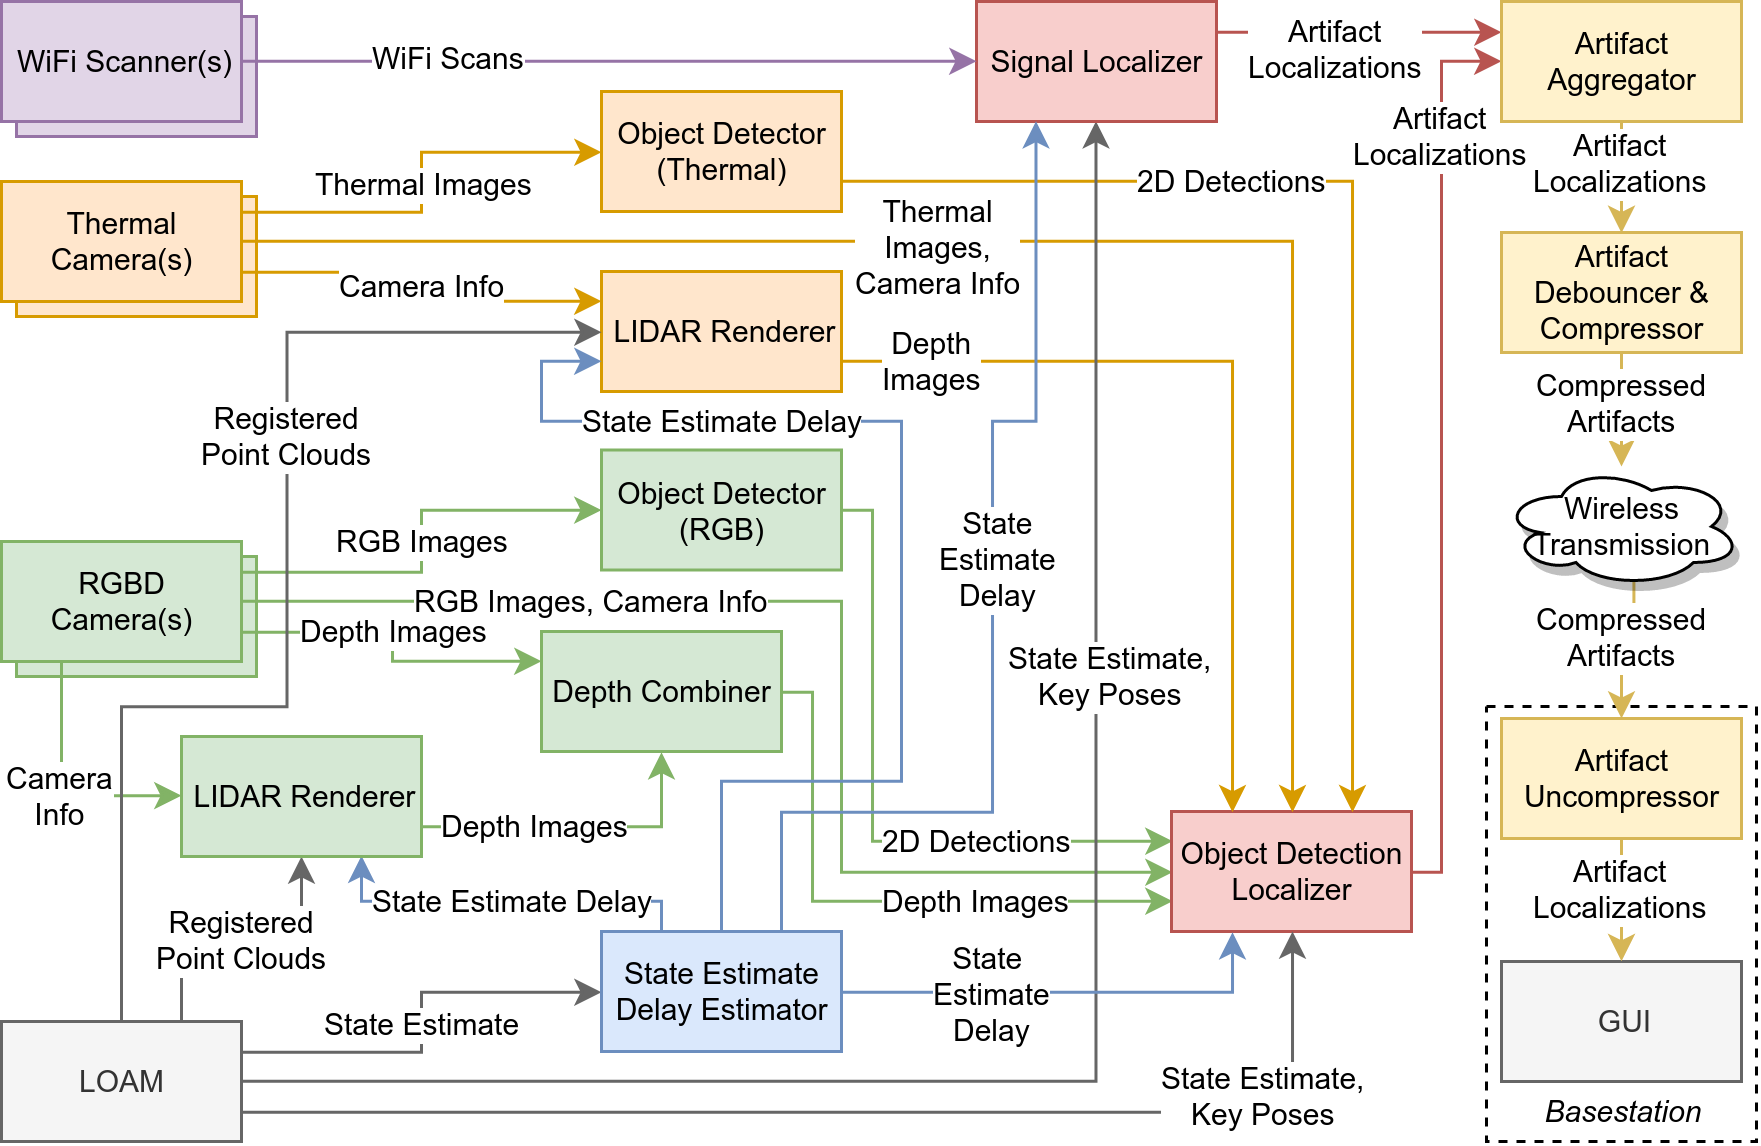
\includegraphics[width=\textwidth]{software_overview.png}
	\caption{Artifact detection and localization software diagram}
	\label{software_overview}
\end{figure}

% TODO(vasua): A better figure for what is inside an artifact localization?
The pipeline consists of 2 major modules - the Signal Localizer and the Object Detection Localizer. Each module takes in various sensor data and produces artifact localizations, which are 3d coordinates in the robot's map frame that are believed to correspond to a desired artifact. These artifact localizations may contain additional evidence to be displayed to the human supervisor, such as images or point clouds of the artifact and surrounding environment. Artifact localizations from both modules are combined inside the Artifact Aggregator and then transmitted to the base station to be displayed on the GUI. The human supervisor inspects artifacts displayed on the GUI and reports valid ones to DARPA.

\section{LOAM Overview}

One of the assumptions made during the initial design phases of the software pipeline was that LOAM would be the state estimation system used on all of our payloads. This simplified the development of the artifact detection and localization pipeline as we only needed to develop and test against a single state estimation system. The relevant interface details of LOAM (in the form of ROS frames and topics) are given below:

\begin{description}
	\item[/sensor] This is the robot's local frame, and is coincident with the Velodyne LIDAR's frame.
	\item[/sensor\_init] The fixed frame used as the base for LOAM's odometry.
	\item[/map] The world frame, which is initially coincident with sensor\_init but can change after loop closures.
	\item[/key\_pose\_to\_map] LOAM creates a series of key poses as the robot traverses the environment. These key poses are generated approximately every 2 meters of the robot's path. Each key pose is given a unique ID, starting from 0. The key pose is published relative to the /map frame.
	\item[/key\_pose\_path] When LOAM detects a loop closure, it corrects the key poses and publishes a new list of key pose IDs and poses.
	\item[/velodyne\_cloud\_registered] The laser scan from the Velodyne LIDAR is aligned to previous scans and published on this topic at 5 Hz. Contrary to key poses, registered scans are published on this topic even when the robot is stationary. The scans are registered in the /sensor\_init frame and accumulate drift over time, but are locally smooth.
	\item[/integrated\_to\_map] The 6DOF pose of the /sensor frame is published on this topic at 200 Hz. The pose is corrected by loop closures and thus does not accumulate significant drift, but may be discontinuous locally.
\end{description}

\section{Object Detector (RGB)}

TODO

\section{Object Detector (Thermal)}

TODO

\section{LIDAR Renderer}

TODO

\section{Depth Combiner}

TODO

\section{Object Detection Localizer}

TODO

\section{WiFi Scanner}

TODO

\section{Signal Localizer}

TODO

\section{State Estimate Delay Estimator}

TODO

\section{Artifact Aggregator}

TODO

\section{Artifact Debouncer \& Compressor}

TODO

\section{Artifact Uncompressor}

TODO

\section{GUI}